% Numbers from results/line_eval_baseline.json (scripts/evaluate_lines.py --extra_preds ...).
Table~\ref{tab:baseline} compares the baseline with our models on all 6,145 test lines. Every
system decodes under the same calibrated length bound, so none exceeds it.

\begin{table}[H]
\centering\small
\caption{External baseline vs.\ our models (test books, 6,145 lines). Lower is better for CER
and \INF\ CER; higher for the rest. ``First word'' is the accuracy of the first word of the
completion.}
\label{tab:baseline}
\begin{tabular}{@{}lccccc@{}}
\toprule
System & \READ\ acc & \INF\ CER & CER & First word & First word @5\
\midrule
LLM only (Qwen2.5-1.5B)          & 0.127 & 0.988 & 0.969 & 0.076 & 0.085\
OCR + LLM (TrOCR + Qwen2.5-1.5B) & 0.657 & 0.948 & 0.876 & 0.386 & 0.397\
Ours, text only (t5-base)        & 0.361 & 0.741 & 0.702 & 0.293 & 0.414\
Ours, full (t5-small)            & \textbf{0.700} & 0.768 & 0.699 & 0.401 & 0.523\
Ours, full (t5-base)             & 0.660 & \textbf{0.717} & \textbf{0.656} & \textbf{0.418} & \textbf{0.553}\
\bottomrule
\end{tabular}
\end{table}

\begin{figure}[H]
\centering
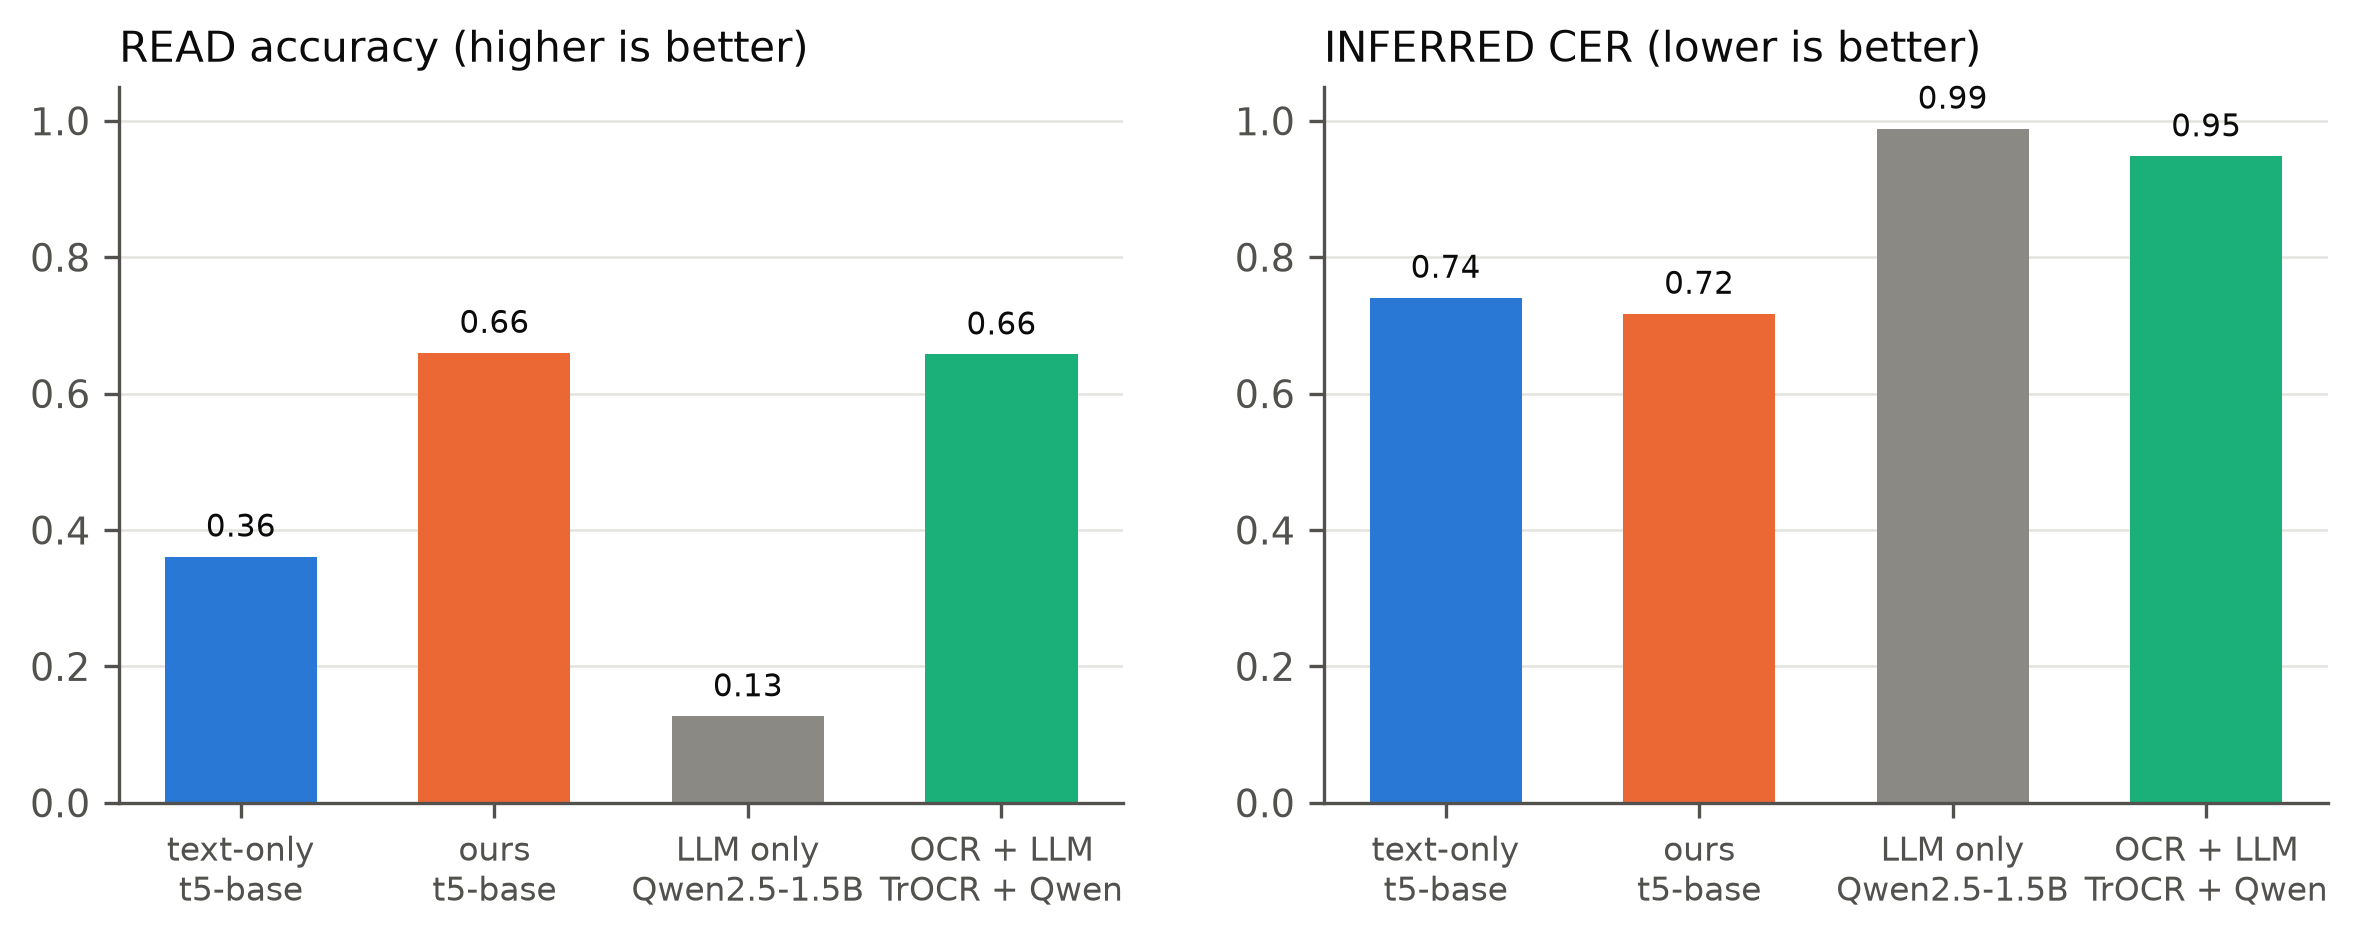
\includegraphics[width=\linewidth]{fig_baseline.png}
\caption{\READ\ accuracy and \INF\ CER of the external baseline and our models.}
\label{fig:baseline}
\end{figure}

Three results stand out (paired bootstrap, 1,000 resamples).
\begin{itemize}[leftmargin=2em,itemsep=1pt]
\item \textbf{Reading faded characters.} With OCR, the baseline reads the faded characters about
as well as our t5-base model (\READ\ accuracy 0.657 vs.\ 0.660; difference not significant,
$p=0.38$). A strong pretrained OCR model can do this step, which supports our finding that this
part of the task is reading, not guessing.
\item \textbf{Guessing the burnt part.} Our full model is far better here (\INF\ CER 0.717 vs.\
0.948, $p<0.001$; overall CER 0.656 vs.\ 0.876). Without task training, the larger LLM tends to
fill the whole available space (37.8\% of its completions are longer than the true ending, against
2.4\% for ours) and rarely reproduces the exact ending (exact match 1.4\% vs.\ 10.3\%).
\item \textbf{The image matters for the LLM too.} Without OCR the LLM gets the first word right
only 7.6\% of the time; with it, 38.6\%. Even our text-only model beats the LLM-only baseline on
every measure (CER 0.702 vs.\ 0.969).
\end{itemize}

Qwen2.5 may have seen Project Gutenberg text during pre-training, which would favour the
baseline. That it still trails our models suggests the gap comes from training on the task
(learning where lines end and how to use the length bound), not from model size.
